\chapter{Studying the Higgs boson through vector boson scattering at CMS}
\begin{aquote}{Peter Higgs, Edinburgh University press conference, 2012}
    It's very nice to be right sometimes.
\end{aquote}

\section{New physics and the Higgs boson}
The stage is set: over a century of particle physics has yielded a beautiful theory of \textit{almost} everything, the Standard Model, and a grand coalition of nations has built the largest and most complex scientific instrument in human history, the LHC, to test it. 
The most recent act in this drama concluded in 2012, when the Higgs boson was discovered at CMS and ATLAS~\cite{CMSdisc, ATLASdisc}. 
In the years following its discovery, the LHC experiments have measured many of its properties to great precision and found no significant deviations from SM predictions~\cite{NatureHiggsCMS2022, NatureHiggsATLAS2022}. 
Nevertheless, the confounding mysteries still surrounding the Higgs boson at the time of writing suggest that there may be some beyond Standard Model (BSM) physics that is not yet understood. 
Given the existential importance of the Higgs boson, this kind of new physics would have profound implications towards a better understanding of the past, present, and future of the entire universe. 

There are many educated guesses, called theories, aimed at addressing the open questions involving the Higgs boson. 
Some guess at the existence of yet-undiscovered particles that also interact with the Higgs boson\footnotemark{}, and experimentalists can search for their existence directly: either by looking for the SM particles that they might decay into, or by checking for what is missing after everything is else accounted for. 
\footnotetext{This is not an unlikely guess: dark matter is known to have mass, and it may haved obtained that mass through the Higgs mechanism.}
Experimentalists can also search for new physics indirectly by making precise measurements of SM predictions; any significant deviation from the prediction would poke another hole in the Standard Model or even confirm a prediction of a new theory. 
The physics analyses described in this document both follow the latter strategy.

\subsection{The $\kappa$-framework}
One commonly used framework used to quantify these deviations from the SM is the so-called $\kappa$-framework~\cite{KFrame}, which introduces modifiers $\kappa_X$ to the Higgs boson couplings to some particle $X$:
\begin{equation}
    \kappa_X = \frac{\text{modifed coupling value}}{\text{SM coupling value}}.
\end{equation}
While there are myriad theoretical nuances to the statement above, it is sufficient to state the obvious: $\kappa_X = 1$ represents the SM scenario and significant deviations from 1 represent BSM scenarios. 
The $\kappa$-framework is not the only framework used to understand and quantify modifications to the SM, however, with the most notable alternative being Effective Field Theory~\cite{EFT, DimSix}. 

\subsection{Vector boson scattering}
The dominant Higgs boson production mechanism at the LHC is gluon-gluon fusion through a top quark loop. % TODO: add feynman diagrams, cite PDG?
Through these processes, the Higgs boson was discovered and many of its branching ratios and couplings have been measured precisely. 
However, additional production mechanisms can yield unique insights. 
Enter vector boson scattering\footnotemark{} (VBS), where two quarks scatter off of each other by the exchange of vector bosons. % TODO: add feynman diagram, ideally with "here there be monsters" circle with stuff coming out
\footnotetext{Although VBS specifically implies the production of two vector bosons, while vector boson fusion (VBF) implies the production of a single Higgs or vector boson~\cite{RauchVBSVBF2016}, the names VBS and VBF are used interchangeably; since we are interested in the production of a Higgs boson and one or two vector bosons, the naming is anyway ambiguous.}
This exchange can, in turn, produce a variety of physics, most notably the production of at least one Higgs boson. 
This process also has two important features. 
First, it has a unique signature: the two scattered quarks fly out of the collision back-to-back, typically in the forward regions of the detector (Fig.~\ref{fig:vbs_fireworks}), with a large combined invariant mass. 
Second, but equally important, modifications to the Higgs couplings induce effects that grow with energy~\cite{HiggsWithoutHiggs}---at the LHC, where energy is plentiful, this makes BSM scenarios easier to spot. 

\begin{figure}[htb]
    \centering
    \subfloat{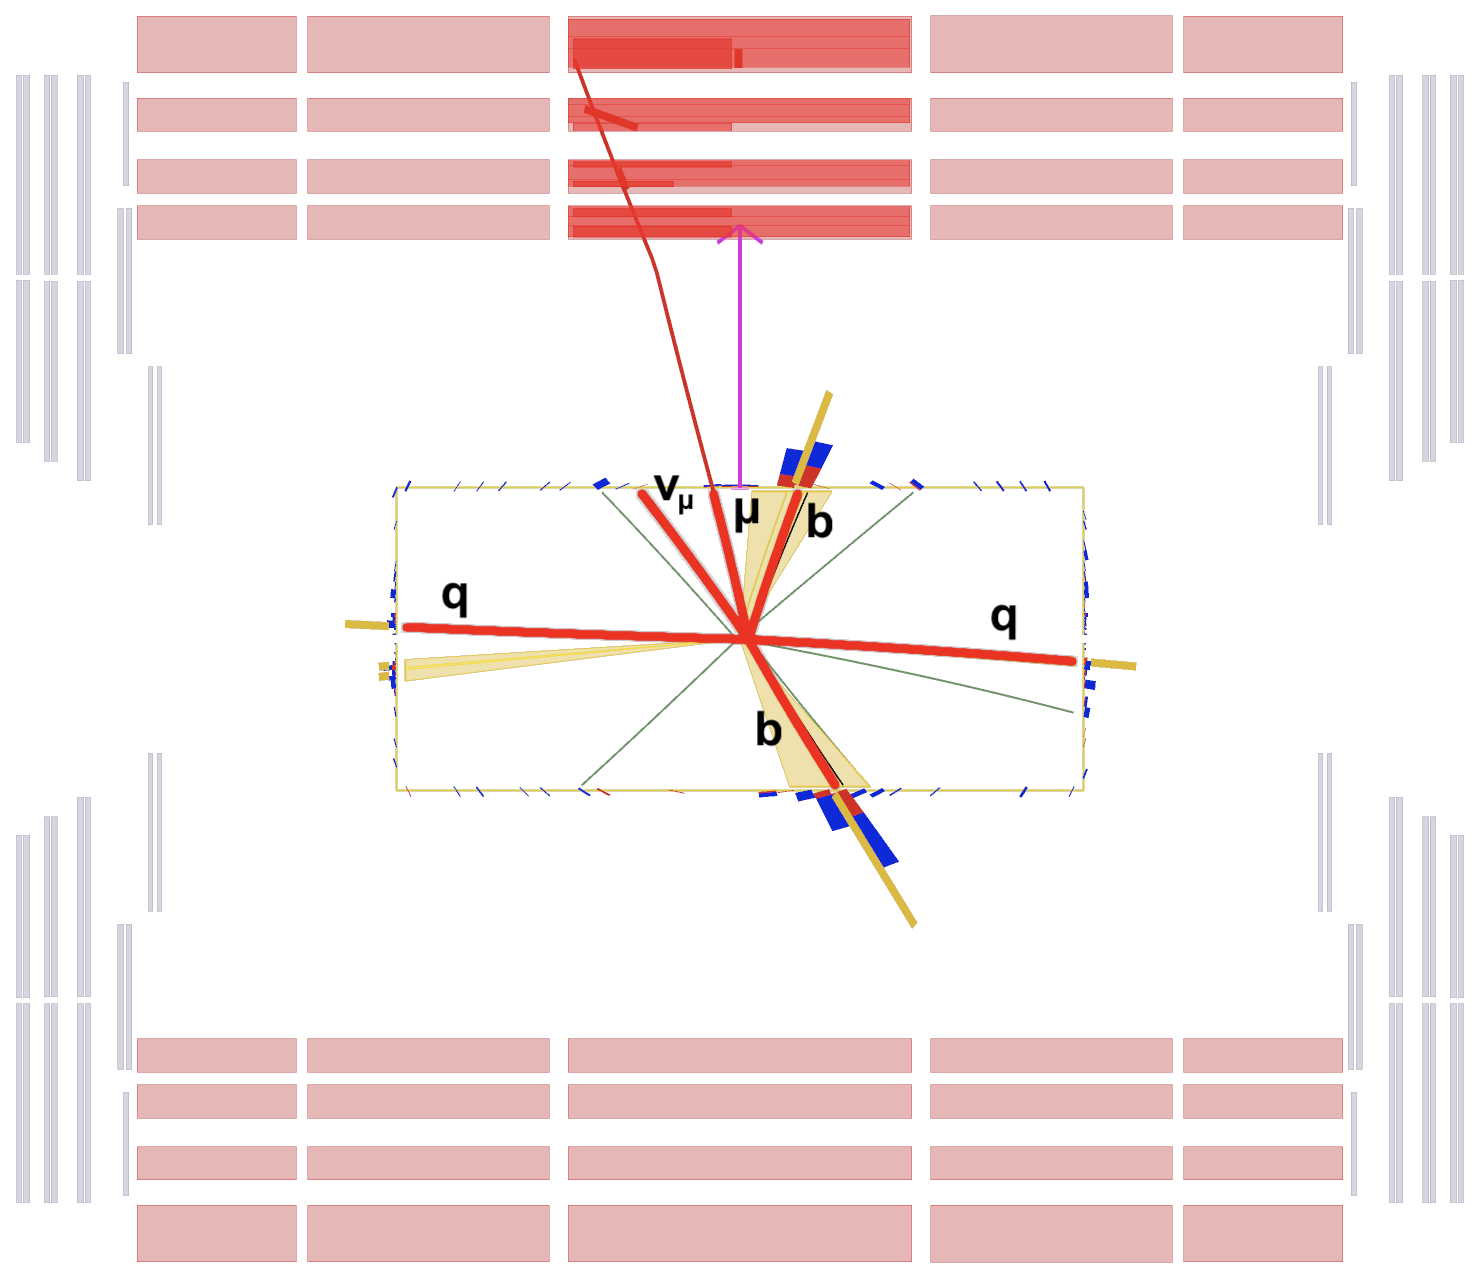
\includegraphics[width=0.45\textwidth]{fig/vbswh/fireworks/signal/vbswh_evt131104_rz_gen_labeled.png}}\qquad
    \subfloat{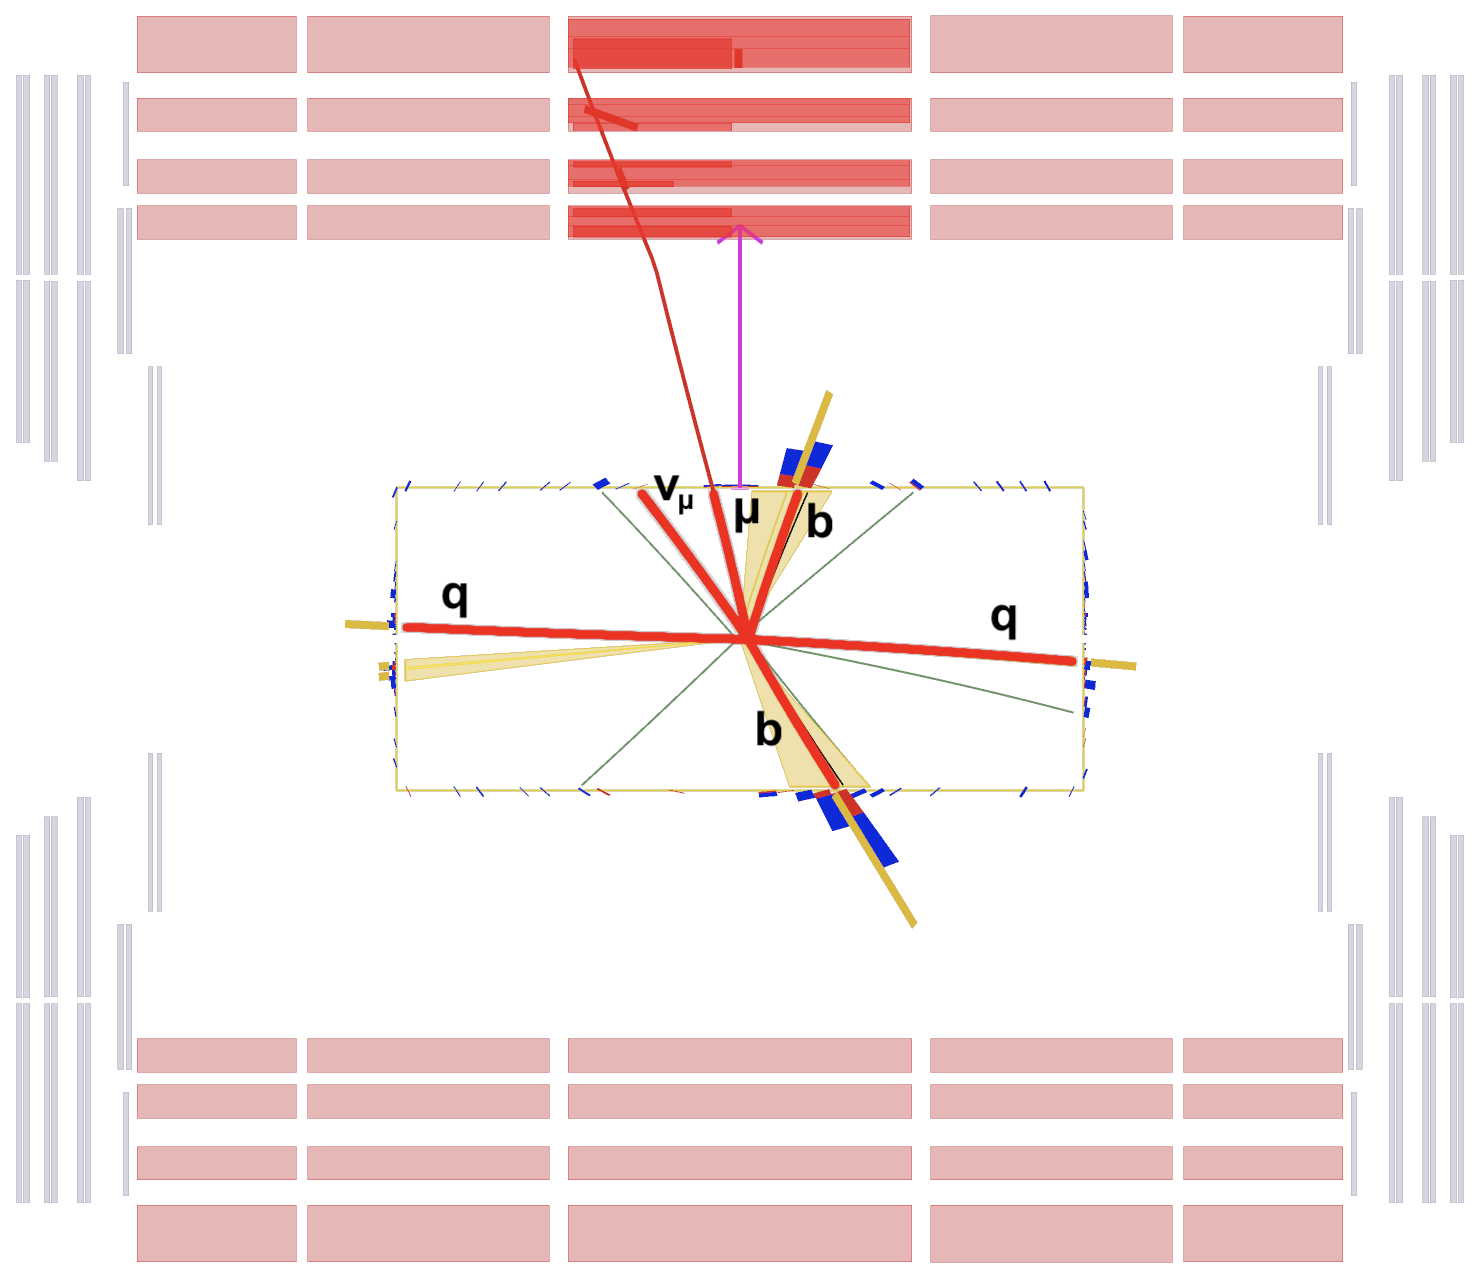
\includegraphics[width=0.45\textwidth]{fig/vbswh/fireworks/signal/vbswh_evt131104_rz_gen_labeled.png}}
    \caption{
        Event display for a simulated VBS WH signal event. 
        The event is shown in the x-y plane (left) and x-z plane (right), and the final-state particles (thick red lines) are labeled with their true labels. 
        Two VBS jets can be seen very near to the beamline, going in either direction in $z$. 
    }
    \label{fig:vbs_fireworks}
\end{figure}

\subsection{Search strategy}

\section{Reconstruction}
\subsection{Leptons}
\subsection{Jets}
\subsubsection{Jets originating from VBS quarks}
\subsubsection{Jets originating from b quarks}

\section{Simulation}

\section{Event selection}
In order to isolate the signal, we must place a set of selections on our data that prefer events that look like signal. 
We do this in a particular order, however, because of the sheer size of our data. 
\subsection{Triggers}
\subsection{Signal regions}
\subsection{Control regions}
\subsection{Background estimation}

\section{Systematic uncertainties}
Since the background estimation strategy is data-driven, the systematics on the Monte Carlo, which are more numerous, only need to be evaluated for the signal yield. 
Most sources of systematic uncertainty are derived by varying individual theoretical scales and experimental corrections by one standard deviation and taking the maximal difference in yield as the error. 
In particular, the corrections and their uncertainties are typically derived centrally in order to augment the efficiency of a specific selection in MC to match that measured in data.
In general, these corrections are applied as an event weight $w$, such that the weighted contribution $W$ of each raw Monte Carlo event is given by the product of the event weights for that same event. 
The yield in a given signal region $y$ containing $N$ raw Monte Carlo events is therefore given by
\begin{equation}
    y = \sum_{i = 1}^{N}W_i
\end{equation}
Then, the yield $y_{var}$ is computed after applying a systematic variation (up or down) of each source of systematic uncertainty independently:
\begin{equation}\label{eq:systs}
    y_{var} = \sum_{i = 1}^{N}W_i\times\frac{w_{var}}{w}
\end{equation}
Finally, the maximum of the percent differences $\delta_{up}$ or $\delta_{down}$ are taken as the systematic uncertainty for that source, where
\begin{equation}
    \delta_{var} = \bigg| 1-\frac{y_{var}}{y} \bigg|
\end{equation}

\section{Statistical interpretation}
\subsection{Maximum likelihood estimate}
